\hypertarget{adat__devel_2lib_2ensem_2ensem__primitive_8h}{}\section{/\+Users/archanar/\+Kinematic\+\_\+factor/adat\+\_\+devel/lib/ensem/ensem\+\_\+primitive.h File Reference}
\label{adat__devel_2lib_2ensem_2ensem__primitive_8h}\index{/Users/archanar/Kinematic\_factor/adat\_devel/lib/ensem/ensem\_primitive.h@{/Users/archanar/Kinematic\_factor/adat\_devel/lib/ensem/ensem\_primitive.h}}


Primitive classes.  


{\ttfamily \#include \char`\"{}ensem\+\_\+primscalar.\+h\char`\"{}}\newline
{\ttfamily \#include \char`\"{}ensem\+\_\+primmatrix.\+h\char`\"{}}\newline
{\ttfamily \#include \char`\"{}ensem\+\_\+primvector.\+h\char`\"{}}\newline
{\ttfamily \#include \char`\"{}ensem\+\_\+primseed.\+h\char`\"{}}\newline
{\ttfamily \#include \char`\"{}ensem\+\_\+primcolormat.\+h\char`\"{}}\newline
{\ttfamily \#include \char`\"{}ensem\+\_\+primcolorvec.\+h\char`\"{}}\newline
{\ttfamily \#include \char`\"{}ensem\+\_\+primgamma.\+h\char`\"{}}\newline
{\ttfamily \#include \char`\"{}ensem\+\_\+primspinmat.\+h\char`\"{}}\newline
{\ttfamily \#include \char`\"{}ensem\+\_\+primspinvec.\+h\char`\"{}}\newline
Include dependency graph for ensem\+\_\+primitive.\+h\+:
\nopagebreak
\begin{figure}[H]
\begin{center}
\leavevmode
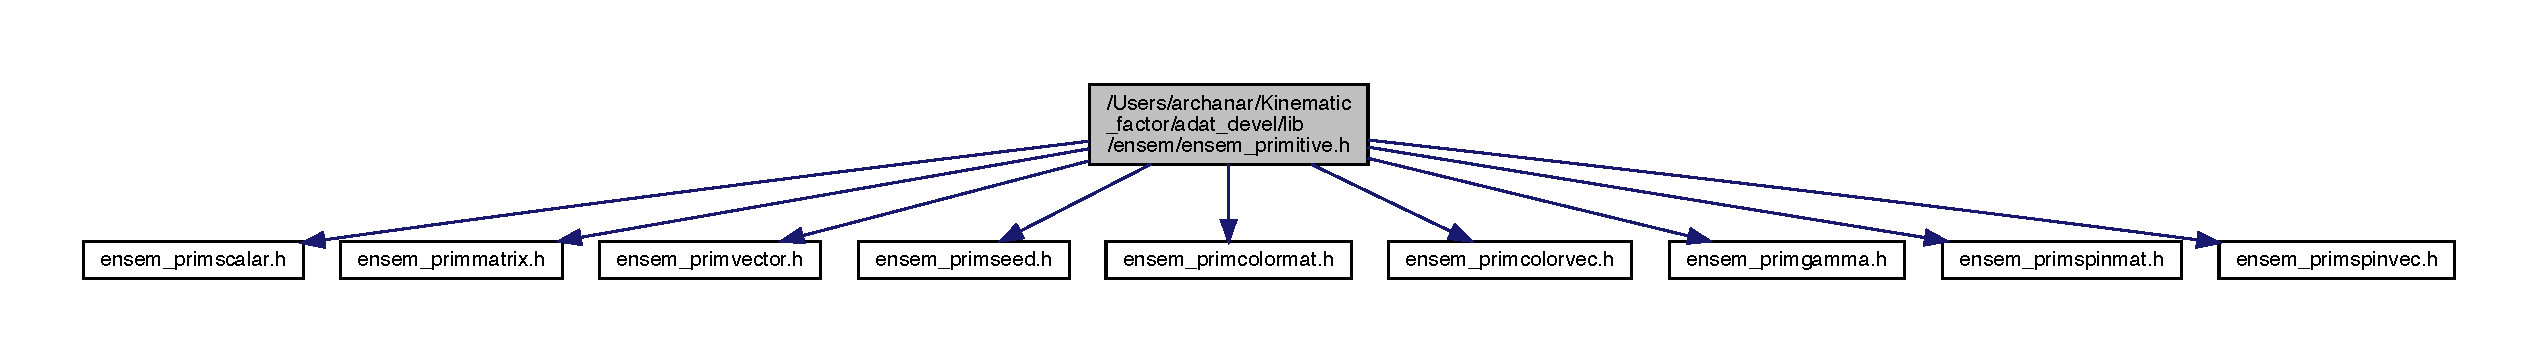
\includegraphics[width=350pt]{de/d22/adat__devel_2lib_2ensem_2ensem__primitive_8h__incl}
\end{center}
\end{figure}
This graph shows which files directly or indirectly include this file\+:
\nopagebreak
\begin{figure}[H]
\begin{center}
\leavevmode
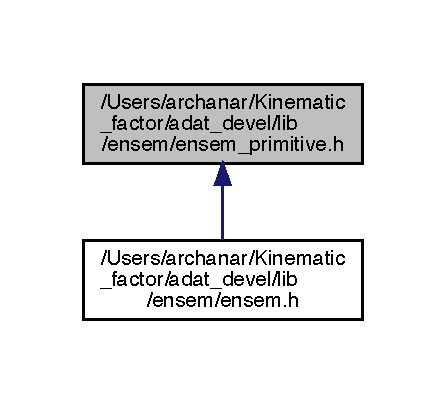
\includegraphics[width=214pt]{d7/d94/adat__devel_2lib_2ensem_2ensem__primitive_8h__dep__incl}
\end{center}
\end{figure}


\subsection{Detailed Description}
Primitive classes. 

Primitives are the various types on the fibers at the lattice sites 